\documentclass[12pt,a4paper]{article}
\usepackage[utf8]{inputenc}
\usepackage[T1]{fontenc}
\usepackage{amsmath}
\usepackage{amsfonts}
\usepackage{amssymb}
\usepackage{graphicx}
\usepackage[indonesian]{babel}
\usepackage[left=2.00cm, right=2.00cm, top=2.00cm, bottom=2.00cm]{geometry}
\usepackage{float} 

\title{Tugas 14 - Pengolahan Sinyal Digital\\
	Disain Filter Digital IIR}

% remove spacing around date:
\usepackage{titling}
\predate{}
\postdate{}
\date{}

\begin{document}
	\maketitle
	\date{}
	\begin{enumerate}
		\item Diketahui frekuensi response dari filter digital yang ditunjukkan oleh Gambar 
		
		\begin{figure}[H]
			\centering
			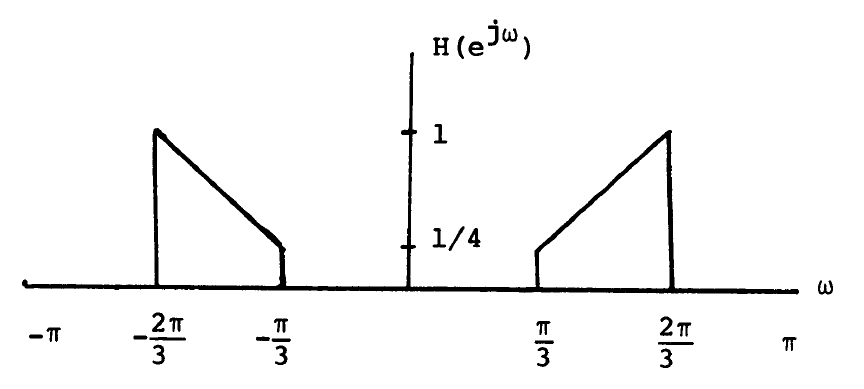
\includegraphics[width=0.7\linewidth]{img/img01}
		\end{figure}
		
		\begin{enumerate}
			\item\label{1a} Tentukan dan gambarkan karakteristik respons frekuensi analog yang, tanpa aliasing, akan dipetakan ke respons frekuensi digital ini ketika dilakukan transformasi impuls invarian.\\
			
			\textbf{Jawaban:}
			
			Tanpa adanya aliasing, transformasi dari analog ke digital frequency response yang sesuai dengan impulse invariance adalah
			
			\begin{figure}[H]
				\centering
				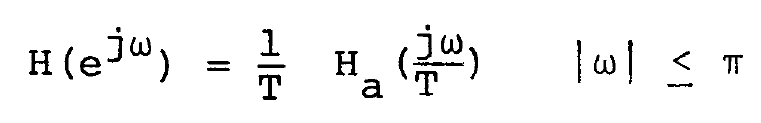
\includegraphics[width=0.5\linewidth]{img/img02}
			\end{figure}
		
			Sehingga, dengan penambahan faktor skala $ 1/T $ maka linear mapping antara frekuensi analog dan frekuensi digital adalah
			
			\begin{figure}[H]
				\centering
				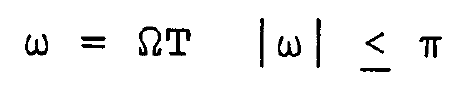
\includegraphics[width=0.3\linewidth]{img/img03}
			\end{figure}
			
			Response frekuensi analog yang diinginkan dapat diperoleh dengan cara merefleksikan response frekuensi digital melalui transformasi berikut
			
			\begin{figure}[H]
				\centering
				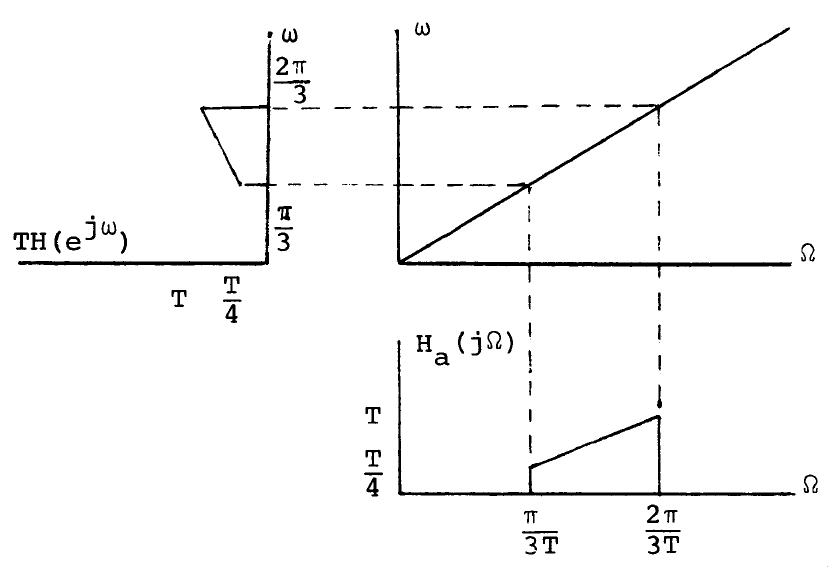
\includegraphics[width=0.8\linewidth]{img/img04}
			\end{figure}
		
			\item Gambarkan frekuensi response analog yang akan memetakan response frekuensi digital ini ketika diberikan transformasi bilinear.\\
			
			\textbf{Jawaban:}
			
			Untuk transformasi biliniear, transformasi antara frekuensi analog dan digital adalah
			
			\begin{figure}[H]
				\centering
				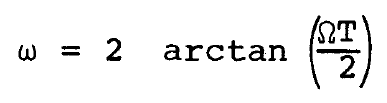
\includegraphics[width=0.3\linewidth]{img/img05}
			\end{figure}
			
			Sehingga, caranya sama seperti jawaban soal nomer (\ref{1a}), kita memperoleh respons frekuensi analog yang sesuai dengan mencerminkan respons frekuensi digital melalui transformasi seperti ini:
			
			\begin{figure}[H]
				\centering
				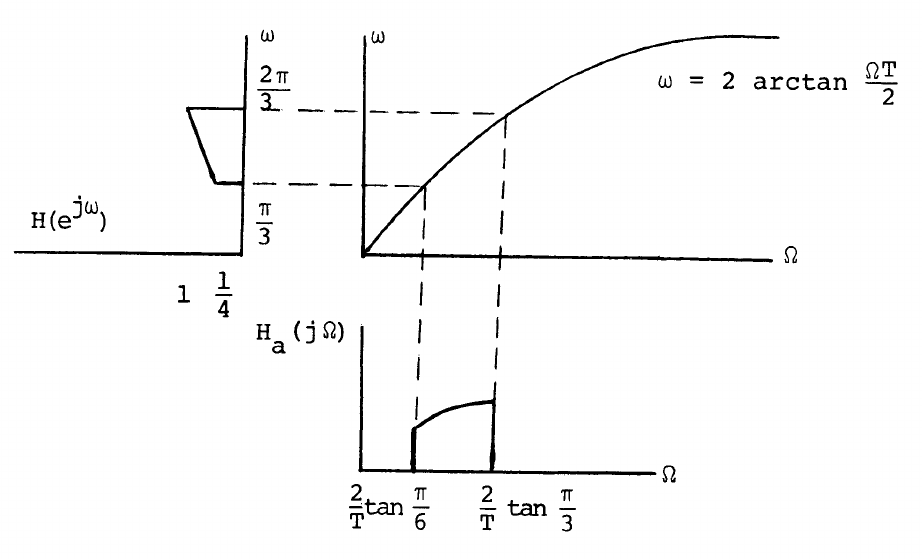
\includegraphics[width=0.8\linewidth]{img/img06}
			\end{figure}
		
		\end{enumerate}
		
	\end{enumerate}
\end{document}